\documentclass[11pt]{article}
\usepackage{emptypage}
\usepackage{cite}
\usepackage{amsmath,amssymb,amsfonts}
\usepackage{caption}
\usepackage{subcaption}
\usepackage{tabularx}
\usepackage{pifont}
\usepackage{siunitx}
\usepackage[explicit]{titlesec}
\usepackage[bookmarks=true]{hyperref}
\usepackage{bookmark}
\usepackage{svg}
\usepackage{amsmath}
\usepackage{listings}
\usepackage{graphicx}
\usepackage{textcomp}
\usepackage{xcolor}
\usepackage{makecell}
\usepackage{float}
\usepackage{stfloats}
\usepackage{authblk}
\usepackage{acro}%by islam
\usepackage[margin=3cm]{geometry}
\usepackage{algorithm2e}
% Drawing
\usepackage{tikz}
% Tikz Library
\usetikzlibrary{calc, quotes, angles}
% Notation
\usepackage{physics, bm}
\usepackage{pgfplots}
\usetikzlibrary{decorations.markings}
\usetikzlibrary{shapes, arrows}
\usepackage{tikz-3dplot}
\usepackage{physics}
\usepackage[outline]{contour} % glow around text
\usepackage{subcaption}

\usepackage{nomencl}
\usepackage{siunitx}
\usepackage{hyperref}
\makenomenclature
\hypersetup{
    colorlinks=true,
    urlcolor=blue,
}
%% This will add the subgroups
%----------------------------------------------
\usepackage{etoolbox}
\renewcommand\nomgroup[1]{%
  \item[\bfseries
  \ifstrequal{#1}{A}{Physics Constants}{%
  \ifstrequal{#1}{B}{Number Sets}{%
  \ifstrequal{#1}{C}{Other Symbols}{}}}%
]}
%----------------------------------------------

%% This will add the units
%----------------------------------------------
\newcommand{\nomunit}[1]{%
\renewcommand{\nomentryend}{\hspace*{\fill}#1}}
%----------------------------------------------


\colorlet{veccol}{green!50!black}
\colorlet{projcol}{blue!70!black}
\colorlet{myblue}{blue!80!black}
\colorlet{myred}{red!90!black}
\colorlet{mydarkblue}{blue!50!black}
\tikzset{>=latex} % for LaTeX arrow head
\tikzstyle{proj}=[projcol!80,line width=0.08] %very thin
\tikzstyle{area}=[draw=veccol,fill=veccol!80,fill opacity=0.6]
\tikzstyle{vector}=[-stealth,myblue,thick,line cap=round]
\tikzstyle{unit vector}=[->,veccol,thick,line cap=round]
\tikzstyle{dark unit vector}=[unit vector,veccol!70!black]
\usetikzlibrary{angles,quotes} % for pic (angle labels)
\contourlength{1.3pt}














\title{Space Systems Engineering Assignment 3}
\author[1]{Mohamed Fawzi}
\author[2]{Islam Zaid}
\affil[1]{Aerospace Department, Khalifa University\\100064444@ku.ac.ae}
\affil[2]{Aerospace Department, Khalifa University\\islam.zaid@ku.ac.ae}
\date{}





% \begin{acronym}[IFR] % Give the longest label here so that the list is nicely aligned
% \acro{IFR}{Inertial Frame of Reference}
% \acro{TLA}{Three Letter Acronym}
% \end{acronym}

\DeclareAcronym{IFR}{
  short=IFR,
  long=Inertial Frame of Reference,
}

\DeclareAcronym{FOV}{
  short=FOV,
  long=Field of View,
}

%%%%%%%%%%%%%%%%%%%%%%%%%%%%%%%%%%%%%%%%%%%%%%%%%%%%%%%%%%%%%%%%%%%%
\begin{document}
\maketitle


\section{Introduction} 
\indent In this report, a thermal model was made on MATLAB to analyze the thermal effects of solar radiation, albedo radiation, and planetary radiation on a satellite. The satellite was modeled to be in LEO orbit, with an altitude of 2000km. The orbit of the satellite is perfectly circular, has an eccentricity (e) of 0, and has an orbital period of 128 min. The velocity of the satellite in orbit is 6.88 km/s, and the satellite is modeled as a disc with a surface area of 100 m2 on each side of the disc. The material of the satellite was decided based on the results of multiple materials to assess which material would allow the satellite to have the most ideal temperature.

\indent The main objective of this assignment was to measure and plot the temperature variation of the satellite while it was in orbit around the Earth for a whole year. While taking into consideration different environmental elements and instances, such as reflection of radiation off the surface of the Earth and onto the satellite, and ellipses the satellite will encounter during the simulation period.


\section{Methodology}   
\indent The spatial and temporal aspects of the simulation are detailed to elucidate the modeling and computational processes. Spherical coordinates, specifically ($r,\theta,\psi$), are employed to describe the positions of orbital elements in three-dimensional space, delineating the satellite’s relative location to Earth. Discretization of the Earth’s surface into latitude and longitude intervals is crucial for accurately representing interactions with solar radiation. Dynamically, the Inertial Frame of Reference \ac{IFR} is defined with respect to the sun, facilitating the translation of positions between the Earth, sun, and satellite. The time-dependent rotational dynamics and celestial mechanics are articulated, utilizing orbital elements to encapsulate the satellite’s motion.

\indent The thermal models introduced include calculations for solar radiation flux, albedo radiation, and planetary radiation, considering the complex geometry of the Earth-sun-satellite system. The methodology also elucidates the determination of eclipse conditions based on the angular position between the sun, Earth, and satellite. Integration over discretized Earth surface elements is emphasized for comprehensive assessments of absorbed radiation. However, this study is simplified to represent a simple relative motion in the equatorial plane, but the conceptual structure of the Matlab code is built with the ability to extend the simulation to 3D coordinates with minimal effort.


\subsection{Positioning and Discretization}

Spherical coordinates ($r,\theta,\psi$) are commonly used to describe positions in three-dimensional space. In this project, these coordinates can be associated with the position of the satellite relative to the Earth or surface elements relative to the center of the earth, as shown in Figure \ref{fig:pos}. The radial distance (r) represents the distance from the Earth's center to the satellite, while the polar angle ($\theta$) and azimuthal angle ($\psi$) define the orientation of the satellite in space.

Figure \ref{fig:elm} introduces the concept of discretizing the Earth's surface into small areas, represented by differential changes ($d\theta, d\psi$). In the MATLAB simulation, this discretization is crucial for modeling how different regions on the Earth's surface interact with solar radiation. Each discrete element can be associated with latitude and longitude intervals, allowing us to calculate the varying solar input across the Earth.


\begin{figure}[h]
 \centering
 \begin{subfigure}[b]{0.48\textwidth}
% 3D AXIS with spherical coordinates
\tdplotsetmaincoords{60}{110}
\resizebox{0.6\textwidth}{!}{
\begin{tikzpicture}[scale=4,tdplot_main_coords]
  
  % VARIABLES
  \def\rvec{.8}
  \def\thetavec{30}
  \def\psivec{60}
  
  % AXES
  \coordinate (O) at (0,0,0);
  \draw[thick,->] (0,0,0) -- (1,0,0) node[anchor=north east]{$x$};
  \draw[thick,->] (0,0,0) -- (0,1,0) node[anchor=north west]{$y$};
  \draw[thick,->] (0,0,0) -- (0,0,1) node[anchor=south]{$z$};
  
  % VECTORS
  \tdplotsetcoord{P}{\rvec}{\thetavec}{\psivec}
  \draw[vector,red] (O)  -- (P) node[above right=-2] {P};
  \draw[dashed,myred]   (O)  -- (Pxy);
  \draw[dashed,myred]   (P)  -- (Pxy);
  \draw[dashed,myred]   (Py) -- (Pxy);
  
  % ARCS
  \tdplotdrawarc[->]{(O)}{0.2}{0}{\psivec}
    {anchor=north}{$\psi$}
  \tdplotsetthetaplanecoords{\psivec}
  \tdplotdrawarc[->,tdplot_rotated_coords]{(0,0,0)}{0.4}{0}{\thetavec}
    {anchor=south west}{\hspace{-1mm}$\theta$}

\end{tikzpicture}
}
 \caption{}
 \label{fig:pos}
 \end{subfigure}
 \begin{subfigure}[b]{0.48\textwidth}
% 3D AXIS with spherical coordinates, dA
\tdplotsetmaincoords{60}{110}
\resizebox{0.6\textwidth}{!}{
\begin{tikzpicture}[scale=4,tdplot_main_coords]
  
  % VARIABLE
  \def\rvec{1.0}
  \def\thetavec{35}
  \def\psivec{45}
  \def\dtheta{10}
  \def\dpsi{16}
  \def\sphere#1#2#3{plot[domain=#1]({\rvec*sin(#2)*cos(#3)},{\rvec*sin(#2)*sin(#3)},{\rvec*cos(#2)})}
  \contourlength{0.8pt}
  
  % AXES
  \coordinate (O) at (0,0,0);
  \draw[thick,->] (0,0,0) -- (1.16*\rvec,0,0) node[left=2,below]{$x$};
  \draw[thick,->] (0,0,0) -- (0,1.1*\rvec,0) node[below=2,right=0]{$y$};
  \draw[thick,->] (0,0,0) -- (0,0,1.1*\rvec) node[above]{$z$};
  
  % COORDINATES
  \tdplotsetcoord{P}{\rvec}{\thetavec}{\psivec}
  \tdplotsetcoord{PB}{\rvec}{\thetavec+\dtheta}{\psivec}
  \tdplotsetcoord{PR}{\rvec}{\thetavec}{\psivec+\dpsi}
  \tdplotsetcoord{PBR}{\rvec}{\thetavec+\dtheta}{\psivec+\dpsi}
  
  % CONE
  \draw[veccol!20,very thin] (O)  -- (PBR);
  \draw[veccol!20,very thin] (O)  -- (PR);
  \draw[->,veccol] (O)  -- (P) node[below=5,left=2] {$\vb{r}$};
  \draw[veccol,very thin] (O)  -- (PB);
  
  % PROJECTIONS
  \draw[proj] %\thetavec+\dtheta
    plot[domain=0:90]({\rvec*sin(\x)*cos(\psivec)},{\rvec*sin(\x)*sin(\psivec)},{\rvec*cos(\x)}) coordinate (BL);
  \draw[proj]
    plot[domain=0:90]({\rvec*sin(\x)*cos(\psivec+\dpsi)},{\rvec*sin(\x)*sin(\psivec+\dpsi)},{\rvec*cos(\x)}) coordinate (BR);
  \draw[proj]
    plot[domain=0:90]({\rvec*cos(\x)},{\rvec*sin(\x)},0);
  \draw[proj] (O)  -- (BL); % PBxy
  \draw[proj] (O)  -- (BR); % PBRxy
  \draw[proj] (P)  -- (Pz);
  \draw[proj] (PR)  -- (Pz) node[midway,above=-2,rotate=-24] {\contour{white}{$r\sin\theta$}};
  
  % AREA
  \draw[area]
    plot[domain=0:.99*\dpsi]({\rvec*sin(\thetavec)*cos(\psivec+\x)},{\rvec*sin(\thetavec)*sin(\psivec+\x)},{\rvec*cos(\thetavec)}) --
    plot[domain=0:.99*\dtheta]({\rvec*sin(\thetavec+\x)*cos(\psivec+\dpsi)},{\rvec*sin(\thetavec+\x)*sin(\psivec+\dpsi)},{\rvec*cos(\thetavec+\x)}) --
    plot[domain=.99*\dpsi:0]({\rvec*sin(\thetavec+\dtheta)*cos(\psivec+\x)},{\rvec*sin(\thetavec+\dtheta)*sin(\psivec+\x)},{\rvec*cos(\thetavec+\dtheta)}) --
    plot[domain=.99*\dtheta:0]({\rvec*sin(\thetavec+\x)*cos(\psivec)},{\rvec*sin(\thetavec+\x)*sin(\psivec)},{\rvec*cos(\thetavec+\x)}) --
    cycle;
    
  % MEASURES;
  \draw[<->,proj,thin]
    plot[domain=0:\dpsi]({\rvec*sin(\thetavec+1.11*\dtheta)*cos(\psivec+\x)},{\rvec*sin(\thetavec+1.11*\dtheta)*sin(\psivec+\x)},{\rvec*cos(\thetavec+1.11*\dtheta)})
    node[right=12,below] {\contour{white}{$r\sin\theta\dd{\psi}$}};
  \draw[<->,proj,thin]
    plot[domain=0:\dtheta]({\rvec*sin(\thetavec+\x)*cos(\psivec+1.15*\dpsi)},{\rvec*sin(\thetavec+\x)*sin(\psivec+1.15*\dpsi)},{\rvec*cos(\thetavec+\x)}) 
    node[above=11,right=-3] {$r\dd{\theta}$};
    
  % ANGLES
  \tdplotdrawarc[->]{(O)}{0.35*\rvec}{0}{\psivec}
    {below=-2}{$\psi$}
  \tdplotdrawarc[->]{(O)}{0.45*\rvec}{\psivec}{\psivec+\dpsi}
    {anchor=145,inner sep=1}{\contour{white}{$\dd{\psi}$}}
  \tdplotsetthetaplanecoords{\psivec}
  \tdplotdrawarc[->,tdplot_rotated_coords]{(0,0,0)}{0.36*\rvec}{0}{\thetavec}
    {right=2,above=-1}{$\theta$}
  \tdplotdrawarc[->,tdplot_rotated_coords]{(0,0,0)}{0.54*\rvec}{\thetavec}{\thetavec+\dtheta}
    {left=0.2,above right=-2}{\contour{white}{$\dd{\theta}$}}
  
\end{tikzpicture}
}

    \caption{}
    \label{fig:elm}
 \end{subfigure}

    \caption{(a) Coordinates system,(b) discretization technique}
\end{figure}





\subsection{Dynamics and Celestial Mechanics}
\paragraph{\ac{IFR}} 
The \ac{IFR} is fixed with respect to the sun, where the origin of the axes is the center of the sun. This \ac{IFR} is defined by three unit vectors $\vec{i}, \vec{j}, \vec{k}$ as shown in Figure \ref{fig:ifr}. $\vec{k}$ is normal to the paper and pointing out.

 
\begin{figure}[h]
 
\centering
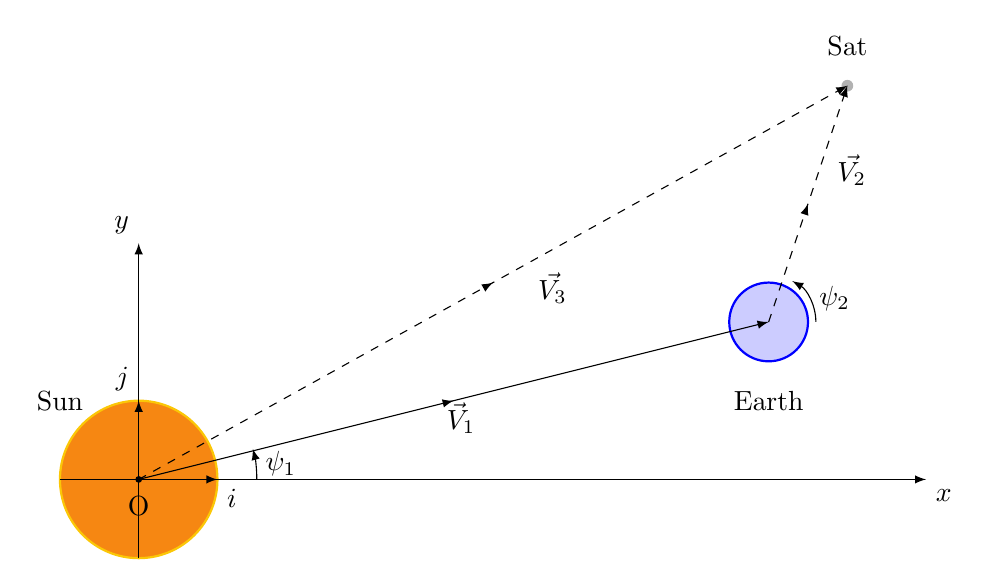
\begin{tikzpicture}[>=latex, decoration={markings, mark=at position 0.5 with {\arrow{>}}}]
    % Coordinates
    \coordinate (sun) at (0,0);
    \coordinate (earth) at (8,2);
    \coordinate (sat) at (9,5);
    \coordinate (A) at (-1,1);
    \coordinate (B) at (8,1);
    \coordinate (C) at (9,5.5);
    
    % Earth
    \draw[thick, fill=yellow!50!red, draw=yellow!80!red] (sun) circle (1);
    % Text
    \node (a) at (A) {Sun};

    % Earth
    \draw[thick, fill=blue!20!white, draw=blue] (earth) circle (0.5);
    % Text
    \node (b) at (B) {Earth};
    
    % Moon
    \node[circle, inner sep=1.5pt, outer sep=2pt, fill=black!30] (MOON) at (sat) {};
    % Text 
    \node (c) at (C) {Sat};
    
    % Lines
    \draw[-latex, postaction={decorate}] (sun) -- (earth) node[pos=.55, below left] {$\vec{V}_{1}$};
    \draw[dashed, -latex, postaction={decorate}] (earth) -- (sat) node[pos=.75, below right] {$\vec{V_2}$};
    \draw[dashed, -latex, postaction={decorate}] (sun) -- (sat) node[pos=.55, below right] {$\vec{V_3}$}; 
    
    % Angles
    \draw[->] (sun) ++(0:1.5) arc (0:15:1.5) node[midway, right] {$\psi_1$};
    \draw[->] (earth) ++(0:0.6) arc (0:60:0.6) node[midway, right] {$\psi_2$};
    
    % Point
    \draw[fill=black] (sun) circle (1pt) node[below, shift={(0,-0.1)}] {$\mathrm{O}$};

    % X and Y axes
    \draw[-latex] (-1,0) -- (10,0) node[below right] {$x$};
    \draw[-latex] (0,-1) -- (0,3) node[above left] {$y$};
    % i and j axes
    \draw[-latex] (0,0) -- (1,0) node[below right] {$i$};
    \draw[-latex] (0,0) -- (0,1) node[above left] {$j$};
\end{tikzpicture}
\caption{\ac{IFR} and vector position of the Earth, and satellite}
\label{fig:ifr}
\end{figure}


 
 
\paragraph{Position vector of the earth w.r.t the sun ($\vec{V_1(\psi_1)}$),}

the vector from the sun to the earth is $\vec{V}_{1}$, which consists of three components in $X, Y, \text{and } Z$ directions. %the initial position of the satellite at $t_0 = 0$ is represented by 
\begin{equation}\label{eq:01}
    \vec{V}_{1}(\psi_{1}) = (r_{1}(\psi_1)) \vec{i} + (0) \vec{j} + (0) \vec{k}\end{equation}
$r_{1}(\psi)$ is the distance between the sun and earth at an angle ($\psi$).

Rotation matrix [$R$] is used to rotate $\vec{V}_{1}$ around the origin of the axes. it results from the multiplication of three rotation matrices ($[R_x], [R_y], \text{ and } [R_z]$) These matrices are 
\begin{equation}
[R_x(\phi)] = \begin{bmatrix}
            1 &0 & 0 \\
            0 & \cos{\phi}& -\sin{\phi} \\
            0 & \sin{\phi}&\cos{\phi}
            \end{bmatrix}
[R_y(\theta)] = \begin{bmatrix}
            cos{\theta} &0 & \sin{\theta} \\
            0 & 1& 0 \\
            -\sin{\theta}&0 & \cos{\theta}
            \end{bmatrix}
[R_z(\psi)] = \begin{bmatrix}
            cos{\psi}  &  -\sin{\psi}  &  0    \\
            \sin{\psi}&   \cos{\psi}    & 0\\
            0          &    0   & 1          
            \end{bmatrix}        
\end{equation}

\begin{equation}\label{eq:11}
[R(\phi, \theta, \psi)]= [R_z(\psi)][R_y(\theta)][R_x(\phi)]
\end{equation}


Since this study targets a simplified model, where the satellite is limited to rotating in the equatorial plane only. Then, no rotation about X, and Y directions. 
Consequently,
\begin{equation}\label{fig:6}
    \phi(t) = \theta(t) = 0 
    \end{equation}
\begin{equation}\label{eq:7}
    [R_x(\phi(t))]=[R_y(\theta(t))]=[eye] .
\end{equation}
By substitution from Equation \ref{eq:11} into Equation \ref{eq:7},
\begin{equation}\label{eq:04}
    [R(\phi, \theta, \psi)] = [eye] [ eye] [R_z(\psi_1(t))]
\end{equation}
\begin{equation}\label{eq:04}
    [R(\psi)] = [R_z(\psi_1(t))]
\end{equation}

\begin{equation}\label{eq:05}
    \vec{V}_1(\psi_1) = [R(\psi_1)] \vec{V}_1(\psi_1)  
\end{equation}

By substitution from Equation \ref{eq:01}, and Equation \ref{eq:04} into Equation \ref{eq:05}

\begin{gather}\label{eq:06}
\vec{V}_1(t) = \begin{bmatrix}
            cos{\psi_1(t)}  &  -\sin{\psi_1(t)}  &  0    \\
            \sin{\psi_1(t)}&   \cos{\psi_1(t)}    & 0\\
            0          &    0   & 1          
            \end{bmatrix}  \begin{bmatrix}
            r_1(t)   \\
            0 \\
             0             
            \end{bmatrix}  
            = \begin{bmatrix}
            r_1(t) . cos{\psi_1(t)}  \\
            r_1(t) . sin{\psi_1(t)} \\
             0             
            \end{bmatrix}
\end{gather}

\paragraph{Position vector of the satellite w.r.t the earth ($\vec{V_2(t)}$),}


Similarly, the satellite is rotating around the earth according to the same governing equations. Considering that the satellite is rotating in a circular path. Then, $r_2(t) = r_2$. Thus,
\begin{equation}
    \vec{V}_2(t) = \begin{bmatrix}
            cos{\psi_2(t)}  &  -\sin{\psi_2(t)}  &  0    \\
            \sin{\psi_2(t)}&   \cos{\psi_2(t)}    & 0\\
            0          &    0   & 1          
            \end{bmatrix}  \begin{bmatrix}
            r_2   \\
            0 \\
             0             
            \end{bmatrix}  
            = \begin{bmatrix}
            r_2 . cos{\psi_2(t)}  \\
            r_2 . sin{\psi_2(t)} \\
             0             
            \end{bmatrix}
\end{equation}
\paragraph{Position vector of the satellite w.r.t the sun ($\vec{V_3(t)}$),}

It is evident from geometry of Figure \ref{fig:ifr} that,
\begin{equation}
    \vec{V_3}(t) = \vec{V_1}(t) + \vec{V_2}(t)
\end{equation}
\begin{equation}
    \vec{V}_3(t)  = 
            \begin{bmatrix}
            r_1(t) . cos{\psi_1(t)}  \\
            r_1(t) . sin{\psi_1(t)} \\
             0             
            \end{bmatrix} 
            +
            \begin{bmatrix}
            r_2 . cos{\psi_2(t)}  \\
            r_2 . sin{\psi_2(t)} \\
             0             
            \end{bmatrix}  
\end{equation}
\begin{equation}
    \vec{V}_3(t)  =  
            \begin{bmatrix}
            r_1(t) . cos{\psi_1(t)} +r_2 . cos{\psi_2(t)}  \\
            r_1(t) . sin{\psi_1(t)} +r_2 . sin{\psi_2(t)} \\
             0                                
            \end{bmatrix} 
\end{equation}


\paragraph{Orbital Elements}


Two-body problem solution of earth-sun system\cite{fortescue2011spacecraft}.
 

In this project, time will be considered as the dependent variable. Thus, the independent variable should be calculated as follows:


\begin{figure}[h]
\centering
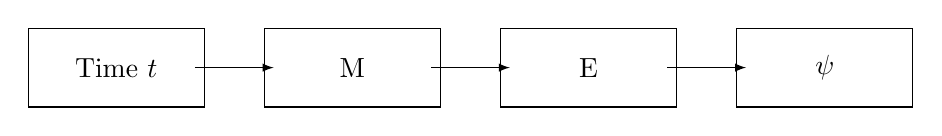
\begin{tikzpicture}
% draw rectangle node
	\node[draw,
		minimum width=2cm,
		minimum height=1cm,
		align=center,
		text width=2cm] at (0,0) {Time $t$};
	\node[draw,
		minimum width=2cm,
		minimum height=1cm,
		align=center,
		text width=2cm] at (3,0) {M};
	\node[draw,
		minimum width=2cm,
		minimum height=1cm,
		align=center,
		text width=2cm] at (6,0) {E};
	\node[draw,
		minimum width=2cm,
		minimum height=1cm,
		align=center,
		text width=2cm] at (9,0) {$\psi$};

    \draw[-latex] (1,0) -- (2,0);
    \draw[-latex] (4,0) -- (5,0);
    \draw[-latex] (7,0) -- (8,0);
\end{tikzpicture}
\caption{Time to State Transition}
\label{fig:2}
\end{figure}




According to the sequence in Figure \ref{fig:2}, the angular position ($\psi$) of the orbital objects could be calculated as a function of a given time (t).

\begin{gather}\label{eq:12}
    M = n t \\
    E-e\sin{E} = M \\
    \tan{\psi/2} = \tan{E/2}\sqrt{\frac{1+e}{1-e}} \\
\end{gather}

Also, the position on the ellipse (r) may be written in terms of ($\psi$) as
\begin{gather}\label{eq:14}
    r = \frac{h^2/\mu}{1+e\cos{\psi_1}}\\
    h^2/\mu = a(1-e^2)
\end{gather}

The periodic time ($\tau$),
 
\begin{equation}
    \tau = 2\pi\sqrt{a^3/\mu}
\end{equation}



\subsection{Thermal Models}
\paragraph{Solar radiation,} The Sun is emitting a constant amount of radiation power ($P$) equal \SI{3.856e26}{\watt}. The solar radiation flux of a point at a distance ($d$) from the center of the earth could be calculated according to Equation \ref{eq:solarflux}.

\begin{equation} \label{eq:solarflux}
    J_s = \frac{Ps}{4\pi d^2}
\end{equation}



\begin{figure}[h]
 
\centering
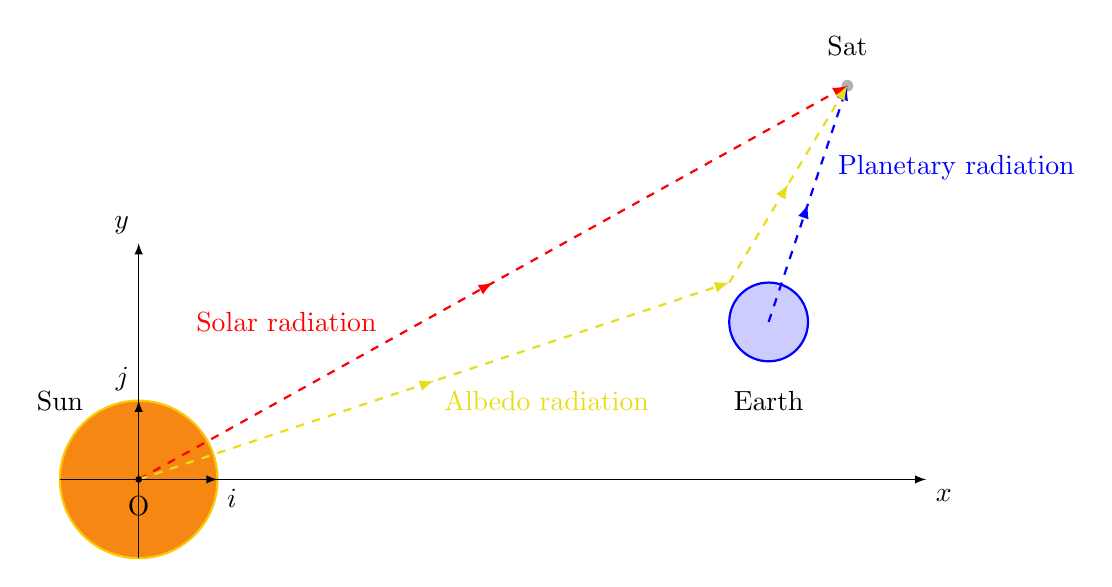
\begin{tikzpicture}[>=latex, decoration={markings, mark=at position 0.5 with {\arrow{>}}}]
    % Coordinates
    \coordinate (sun) at (0,0);
    \coordinate (earth) at (8,2);
    \coordinate (sat) at (9,5);
    \coordinate (A) at (-1,1);
    \coordinate (B) at (8,1);
    \coordinate (C) at (9,5.5);
    
    % Earth
    \draw[thick, fill=yellow!50!red, draw=yellow!80!red] (sun) circle (1);
    % Text
    \node (a) at (A) {Sun};

    % Earth
    \draw[thick, fill=blue!20!white, draw=blue] (earth) circle (0.5);
    % Text
    \node (b) at (B) {Earth};
    
    % Moon
    \node[circle, inner sep=1.5pt, outer sep=2pt, fill=black!30] (MOON) at (sat) {};
    % Text 
    \node (c) at (C) {Sat};
    
    % Lines
    % \draw[-latex, postaction={decorate}] (sun) -- (earth) node[pos=.55, below left] {$\vec{V}_{1}$};
    \draw[dashed, -latex, postaction={decorate},blue,thick] (earth) -- (sat) node[pos=.75, below right] {\textcolor{blue}{Planetary radiation}};
    \draw[dashed, -latex, postaction={decorate},red,thick] (sun) -- (sat) node[pos=.35, above left] {\textcolor{red}{Solar radiation}}; 
    \draw[dashed, -latex, postaction={decorate},yellow!90!black,thick] (sun) -- (7.5,2.5) node[pos=.5, below right] {\textcolor{yellow!90!black}{Albedo radiation}}; 
    \draw[dashed, -latex, postaction={decorate},yellow!90!black,thick] (7.5,2.5) -- (sat) node[pos=.5, below right] {}; 
    
    % Angles
    % \draw[->] (sun) ++(0:1.5) arc (0:15:1.5) node[midway, right] {$\psi_1$};
    % \draw[->] (earth) ++(0:0.6) arc (0:60:0.6) node[midway, right] {$\psi_2$};
    
    % Point
    \draw[fill=black] (sun) circle (1pt) node[below, shift={(0,-0.1)}] {$\mathrm{O}$};

    % X and Y axes
    \draw[-latex] (-1,0) -- (10,0) node[below right] {$x$};
    \draw[-latex] (0,-1) -- (0,3) node[above left] {$y$};
    % i and j axes
    \draw[-latex] (0,0) -- (1,0) node[below right] {$i$};
    \draw[-latex] (0,0) -- (0,1) node[above left] {$j$};
\end{tikzpicture}
\caption{Radiation Modes}
\label{fig:modes}
\end{figure}





The relative motion between the three components—the sun, earth, and satellite—provides the possibility of eclipse conditions, in which the satellite will be outside the visible region of the sun. Consequently, the direct solar radiation will not arrive at the satellite. This case can be captured in the simulation by defining a certain condition that can determine whether the satellite is in an eclipse quantitatively. Equation \ref{eq:psi13} provides the proposed mathematical concept, which is calculated each time step to determine if there is a direct contribution from the sun radiation. Simply stated, does the satellite pass through the field of view \ac{FOV} of the sun?



\begin{figure}[h]
 
\centering
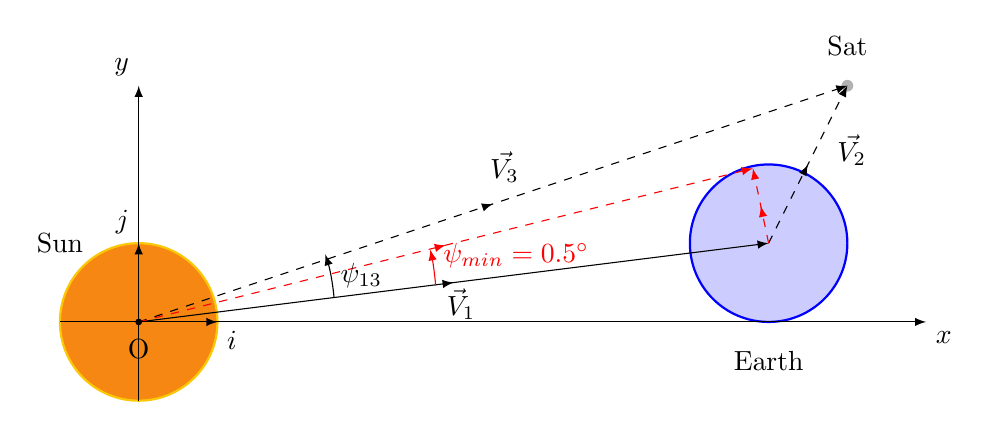
\begin{tikzpicture}[>=latex, decoration={markings, mark=at position 0.5 with {\arrow{>}}}]
    % Coordinates
    \coordinate (sun) at (0,0);
    \coordinate (earth) at (8,1);
    \coordinate (sat) at (9,3);
    \coordinate (A) at (-1,1);
    \coordinate (B) at (8,-0.5);
    \coordinate (C) at (9,3.5);
    
    % Earth
    \draw[thick, fill=yellow!50!red, draw=yellow!80!red] (sun) circle (1);
    % Text
    \node (a) at (A) {Sun};

    % Earth
    \draw[thick, fill=blue!20!white, draw=blue] (earth) circle (1);
    % Text
    \node (b) at (B) {Earth};
    
    % Moon
    \node[circle, inner sep=1.5pt, outer sep=2pt, fill=black!30] (MOON) at (sat) {};
    % Text 
    \node (c) at (C) {Sat};
    
    % Lines
    \draw[-latex, postaction={decorate}] (sun) -- (earth) node[pos=.55, below left] {$\vec{V}_{1}$};
    \draw[dashed, -latex, postaction={decorate}] (earth) -- (sat) node[pos=.75, below right] {$\vec{V_2}$};
    \draw[dashed, -latex, postaction={decorate}] (sun) -- (sat) node[pos=.55, above left] {$\vec{V_3}$}; 
    \draw[dashed, -latex, postaction={decorate},draw=red] (sun) -- (7.8,1.95) node[pos=.55, below right] {};  
    \draw[dashed, -latex, postaction={decorate},draw=red] (earth) -- (7.8,1.95) node[pos=.55, below right] {}; 

    
    % Angles
    \draw[->] (sun) ++(7:2.5) arc (5:18:2.5) node[midway, right] {$\psi_{13}$};
    \draw[->, ,draw=red] (sun) ++(7:3.8) arc (5:12:3.8) node[midway, right, shift={(0,0.15)}] {\textcolor{red}{$\psi_{min}=\SI{0.5}{\degree}$}};
    % \dra1[->] (earth) ++(0:0.6) arc (0:60:0.6) node[midway, right] {$\psi_{min}$};
    
    % Point
    \draw[fill=black] (sun) circle (1pt) node[below, shift={(0,-0.1)}] {$\mathrm{O}$};

    % X and Y axes
    \draw[-latex] (-1,0) -- (10,0) node[below right] {$x$};
    \draw[-latex] (0,-1) -- (0,3) node[above left] {$y$};
    % i and j axes
    \draw[-latex] (0,0) -- (1,0) node[below right] {$i$};
    \draw[-latex] (0,0) -- (0,1) node[above left] {$j$};
\end{tikzpicture}
\caption{Layout of a Critical Eclipse Condition w.r.t $\psi_{min}$}
\label{fig:minangle}
\end{figure}



\begin{equation}\label{eq:psi13}
    \psi_{13} = \arccos{\frac{\vec{V}_1\cdot \vec{V}_3}{\norm{\vec{V}_1}\norm{\vec{V}_3}}}
\end{equation}

\paragraph{Albedo radiation} 
The portion of solar radiation that bounces off a planet's surface and/or atmosphere. This fraction (a) is in the range (0.31–0.39).
\begin{equation}
    \delta Q_{r_{ij}} = I_{i0} dA_i\cos{\phi_i}\times\frac{dA_j \cos{\phi_j}}{d^2}
\end{equation}

Each place on the Earth's surface has different geometrical relationships with respect to the sun and satellite. Thus, it's mandatory to discretize the Earth into a mesh grid to be able to numerically integrate over the Earth's surface to compute the total absorbed radiation by the albedo radiation. The following algorithm is developed to compute the incident radiation from each element on the Earth's surface to the satellite and sum all the Earth's contributions to get the total albedo radiation as described in Algorithm \ref{alg:01}.



\RestyleAlgo{ruled}

%% This is needed if you want to add comments in
%% your algorithm with \Comment
\SetKwComment{Comment}{/* }{ */}

\begin{algorithm}[hbt!]
\caption{Satellite-Element Interaction Algorithm for Albedo Radiation}\label{alg:two}
\label{alg:01}
\KwData{$\vec{V}_{n}$, $\vec{A}_{sat}$,$\vec{V}_{sat/elm}$, $a$, $I_{i0}$}
\KwResult{$Q_a = \iint{I_{i0} dA_i\cos{\phi_i}\times\frac{dA_j \cos{\phi_j}}{d^2}}$}
$\vec{V}_{n} \gets $List of normal vectors on elements\;
$\vec{A}_{sat} \gets $Satellite area Vector\;
$\vec{V}_{sat/elm} \gets$ Position vector of satellite/element\;

    \For{  elm = 1 : numElments }{
        $\cos{\phi_1} = \frac{\vec{V}_{n}(elm) \cdot \vec{V}_{sat/elm}}{\norm{\vec{V}_{n}(elm)}\cdot\norm{\vec{V}_{sat/elm}}}$ \\
        $\cos{\phi_2} = \frac{\vec{A}_{sat} \cdot \vec{V}_{sat/elm}}{\norm{\vec{A}_{sat}}\cdot\norm{\vec{V}_{sat/elm}}}$ \\
        $d = \norm{\vec{V}_{sat/elm}}$\\
        $Q_{a}(elm) = a \times I_{i0} \times \cos{\phi_1}\times \cos{\phi_2}\times 
        A_{sat} \times A_{elm}/d^2$ }
        
    $Q_a = \Sigma_{i=1}^{numElements}{Q_s(i)}  $
\end{algorithm}

\begin{equation}
    \vec{V}_{elm/sat} = \vec{V}_{2} - \vec{V}_{elm}
\end{equation}

\begin{figure}[h]
 
\centering
\begin{tikzpicture}[>=latex, decoration={markings, mark=at position 0.5 with {\arrow{>}}}]
    % Coordinates
    \coordinate (earth) at (0,0);
    \coordinate (sat) at (2,3);
    \coordinate (A) at (-1,1);
    \coordinate (B) at (0,-1.5);
    \coordinate (C) at (2,3.5);
    


    % Earth
    \draw[thick, fill=blue!20!white, draw=blue] (earth) circle (1);
    % Text
    \node (b) at (B) {Earth};
    
    % Moon
    \node[circle, inner sep=1.5pt, outer sep=2pt, fill=black!30] (MOON) at (sat) {};
    % Text 
    \node (c) at (C) {Sat};
    
    % Lines
    % \draw[-latex, postaction={decorate}] (sun) -- (earth) node[pos=.55, below left] {$\vec{V}_{1}$};
    \draw[dashed, -latex, postaction={decorate},green,thick] (earth) -- (sat) node[pos=.60, below right] {\textcolor{green}{$\vec{V_2}$}};
    \draw[dashed, -latex, postaction={decorate},yellow!30!blue,thick] ({cos(135)},{sin(135}) -- (sat) node[pos=.4, above left] {\textcolor{yellow!30!blue}{$\vec{V}_{sat/elm}$}}; 
    \draw[dashed, -latex, postaction={decorate},yellow!50!red,thick] (0,0) --  ({cos(135)},{sin(135}) node[pos=.5,  left] {\textcolor{yellow!50!red}{$\vec{V}_{elm}$}}; 

    % Point
    \draw[fill=yellow!10!red, draw=yellow!10!red] ({cos(135)},{sin(135}) circle (2pt) node[left, shift={(-0.,0)}] {\textcolor{yellow!10!red}{$\mathrm{element}$}};
    % Point
    \draw[fill=yellow!50!red] (sun) circle (1pt) node[below, shift={(0,-0.1)}] {$\mathrm{O}$};

    % X and Y axes
    \draw[-latex] (-1,0) -- (4,0) node[below right] {$x$};
    \draw[-latex] (0,-1) -- (0,3) node[above left] {$y$};
    % i and j axes
    \draw[-latex] (0,0) -- (1,0) node[below right] {$i$};
    \draw[-latex] (0,0) -- (0,1) node[above left] {$j$};
\end{tikzpicture}
\caption{Satellite Position Relative to Earth Surface Elements}
\label{fig:}
\end{figure}


\paragraph{Planetary radiation,} the Earth's temperature drives the planet to emit a radiation power that is proportional to the quadratic of the temperature as shown in Equation \ref{eq:palnet_rad}.

\begin{equation}\label{eq:palnet_rad}
    Q_p = \varepsilon \sigma T^4
\end{equation}


\paragraph{Energy Balance,} the satellite is represented as a node with temperature ($T_{sat}$). Accordingly, the satellite emits a radiation power as shown in Equation \ref{eq:sat_rad}

\begin{equation}\label{eq:sat_rad}
    J_{\text {radiated }} = \varepsilon \sigma T^4
\end{equation}

The satellite has specific values of absorptivity ($\alpha$) and emissivity ($\epsilon$) according to the properties of the surface. Thus, the energy balance can be expressed as follow; 

\begin{equation}
A_\alpha J_{\text {absorbed }}=A_\alpha \alpha J_{\text {incident }}=A_{\varepsilon} J_{\text {radiated }}
\end{equation}


\begin{equation}
J_{\text {incident }} = J_p A_p \alpha +\alpha \left(J_s A_s+J_a A_a\right)
\end{equation}


\begin{equation}
T^4=\frac{A_\alpha}{A_{\varepsilon}} \frac{J_{\text {incident }}}{\sigma}\left(\frac{\alpha}{\varepsilon}\right)
\end{equation} 


\begin{equation}
T^4=\frac{Q}{A_{t o t}(\sigma \varepsilon)}+\frac{J_p A_p}{A_{t o t} \sigma}+\left(\frac{J_s A_s+J_a A_a}{A_{t o t} \sigma}\right) \frac{\alpha}{\varepsilon}
\end{equation}

Q: Generated heat due to the satellite subsystems.


 
\newpage
\section{Results} %MSF&IZ
\indent

\subsection{Sensitivity Analysis}

To track the relationship between the number of elements and the simulation performance, a convergence study is conducted. The Earth's surface was uniformly partitioned into various components along the longitude and latitude axes. With regard to a set of elements (10, 20, 40, and 80), the simulation was executed. Figure \ref{fig:ss} shows the sensitivity study, considering the absorbed radiation and the satellite temperature as probes. Those two values converge at the number of elements of 40 in both the longitude and latitude directions, leading to $1600$ $(40\times40)$ elements in total. According to this study, the number of elements is fixed at 40 in both directions for the following simulations.

\begin{figure}[h]
    \centering
    \begin{subfigure}[b]{0.48\textwidth}
        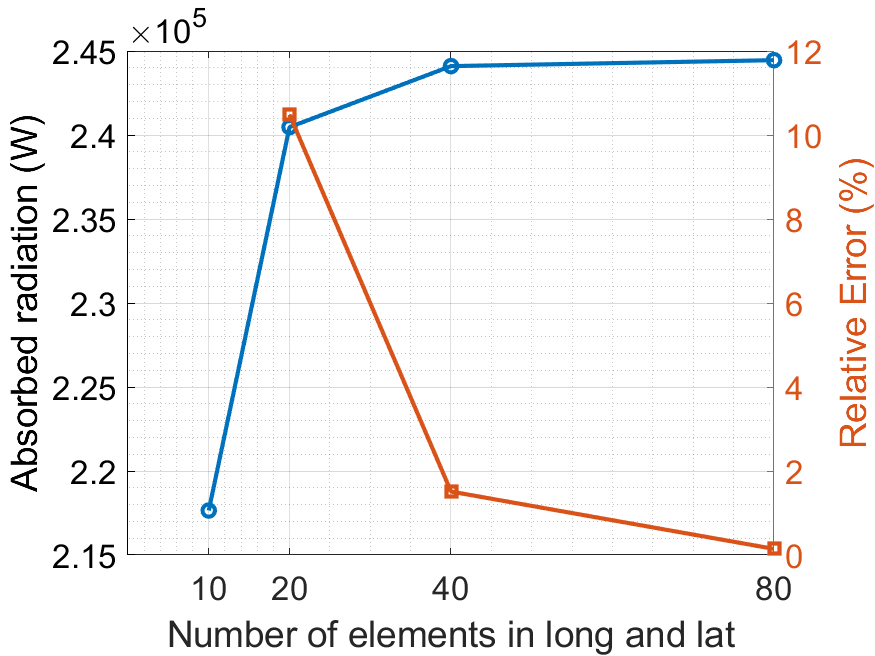
\includegraphics[width = 0.8 \textwidth]{Matlab/Sensitivity/fig_Q_sensitivity_0_180.png}
        \caption{}
        \label{fig:ssa}    
    \end{subfigure}
    \begin{subfigure}[b]{0.48\textwidth}
        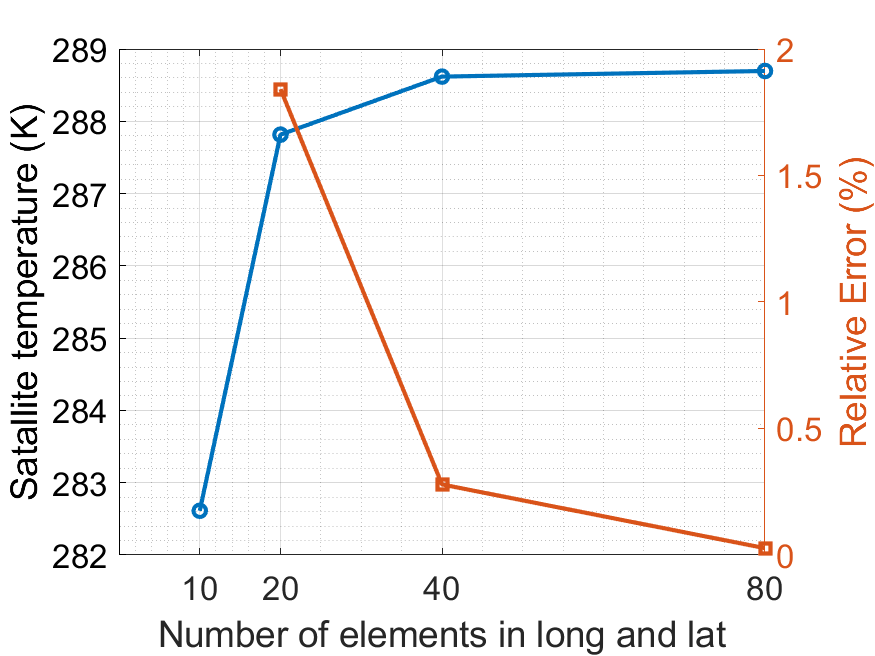
\includegraphics[width = 0.8 \textwidth]{Matlab/Sensitivity/fig_temp_sensitivity_0_180.png}
        \caption{}
        \label{fig:ssb}    
    \end{subfigure}
    \caption{(a) Total absorbed radiation and relative error, (b) satellite temperature and relative error for different number of elements at a satellite position between the sun and the earth.}
    \label{fig:ss}
\end{figure}

\paragraph{Direct solar radiation on the earth surface,} To test the code's performance, each component of the code is tested separately. Thus, the direct radiation from the sun to the earth is computed for each element on the earth's surface. Figure \ref{fig:solar-rad-on-earth} shows the incident radiation on the earth surface, which depends on how far this point is from the sun. The change in the distance (d) of each element on the earth from the sun is very small. Thus, it is expected to get very small differences in the incident radiation power, as evident from the figure where the maximum value and the minimum value are~\textcolor{red}{ X and Y}, respectively.

 
\begin{figure}[h]
    \centering
    \begin{subfigure}[b]{0.48\textwidth}
        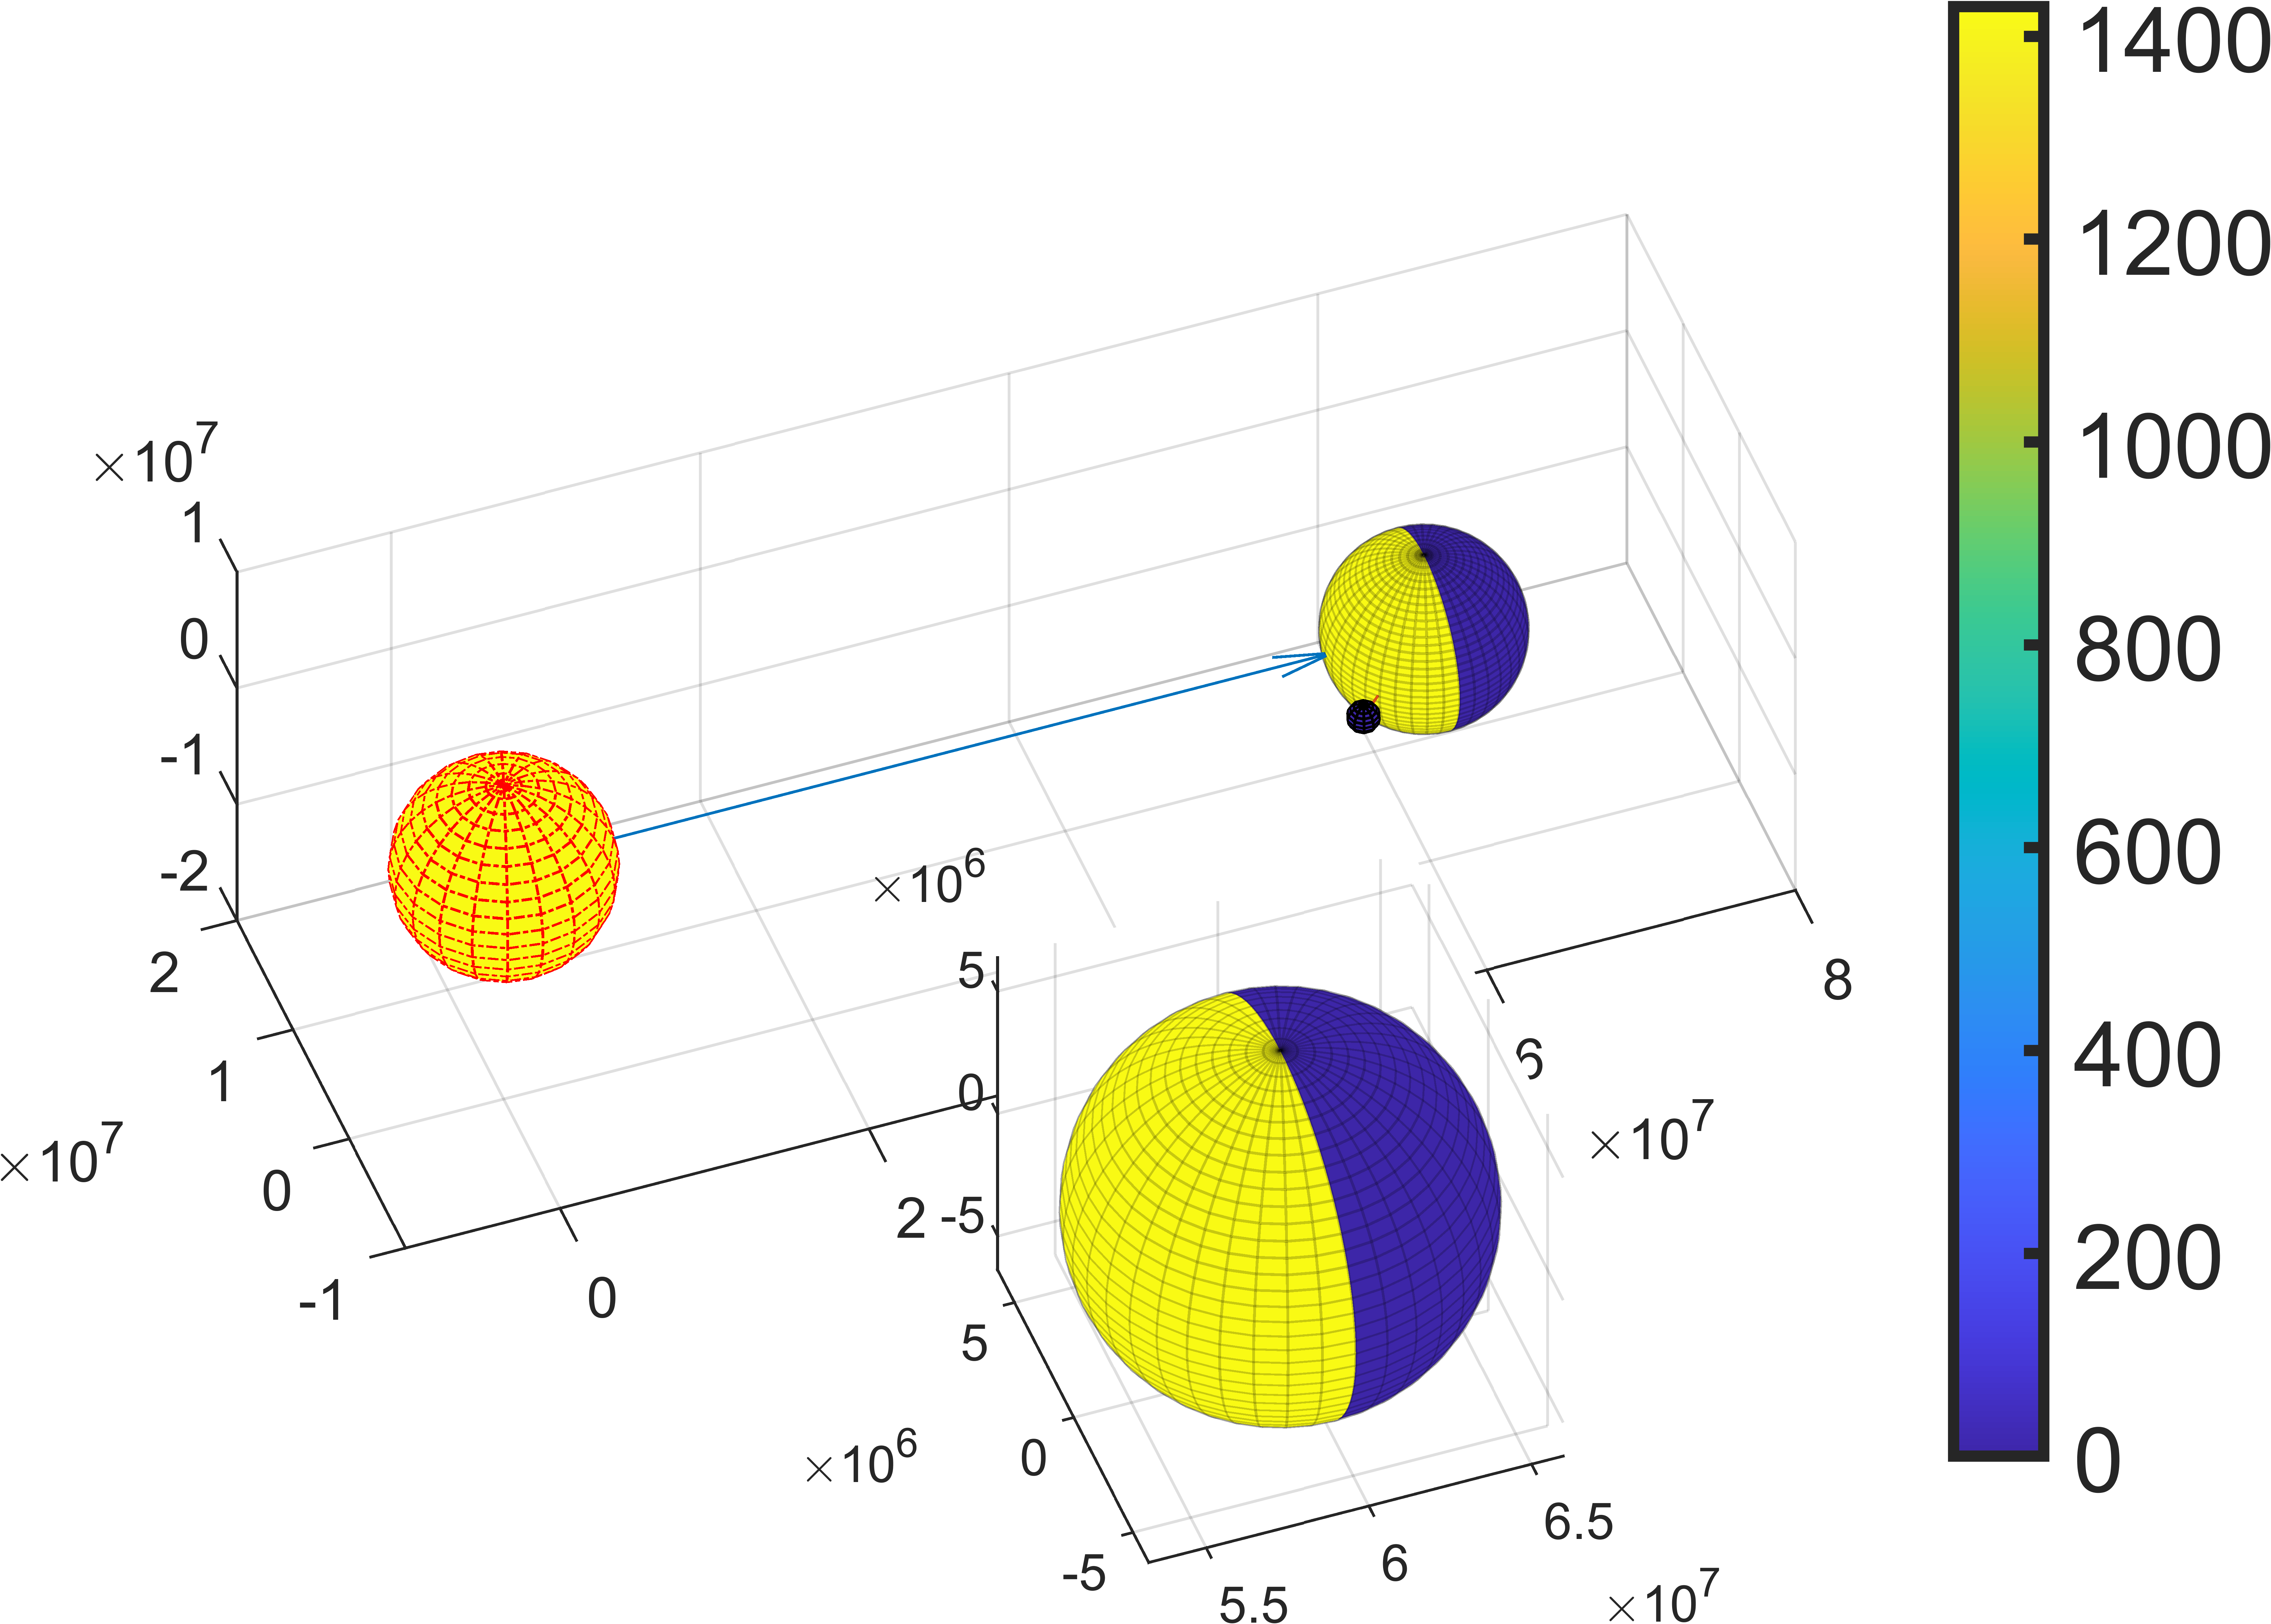
\includegraphics[width=\textwidth]{Matlab/images/inc_sun_rad.png}
        \caption{}
        \label{fig:solar-rad-on-earth}
    \end{subfigure}
    \begin{subfigure}[b]{0.48\textwidth}
        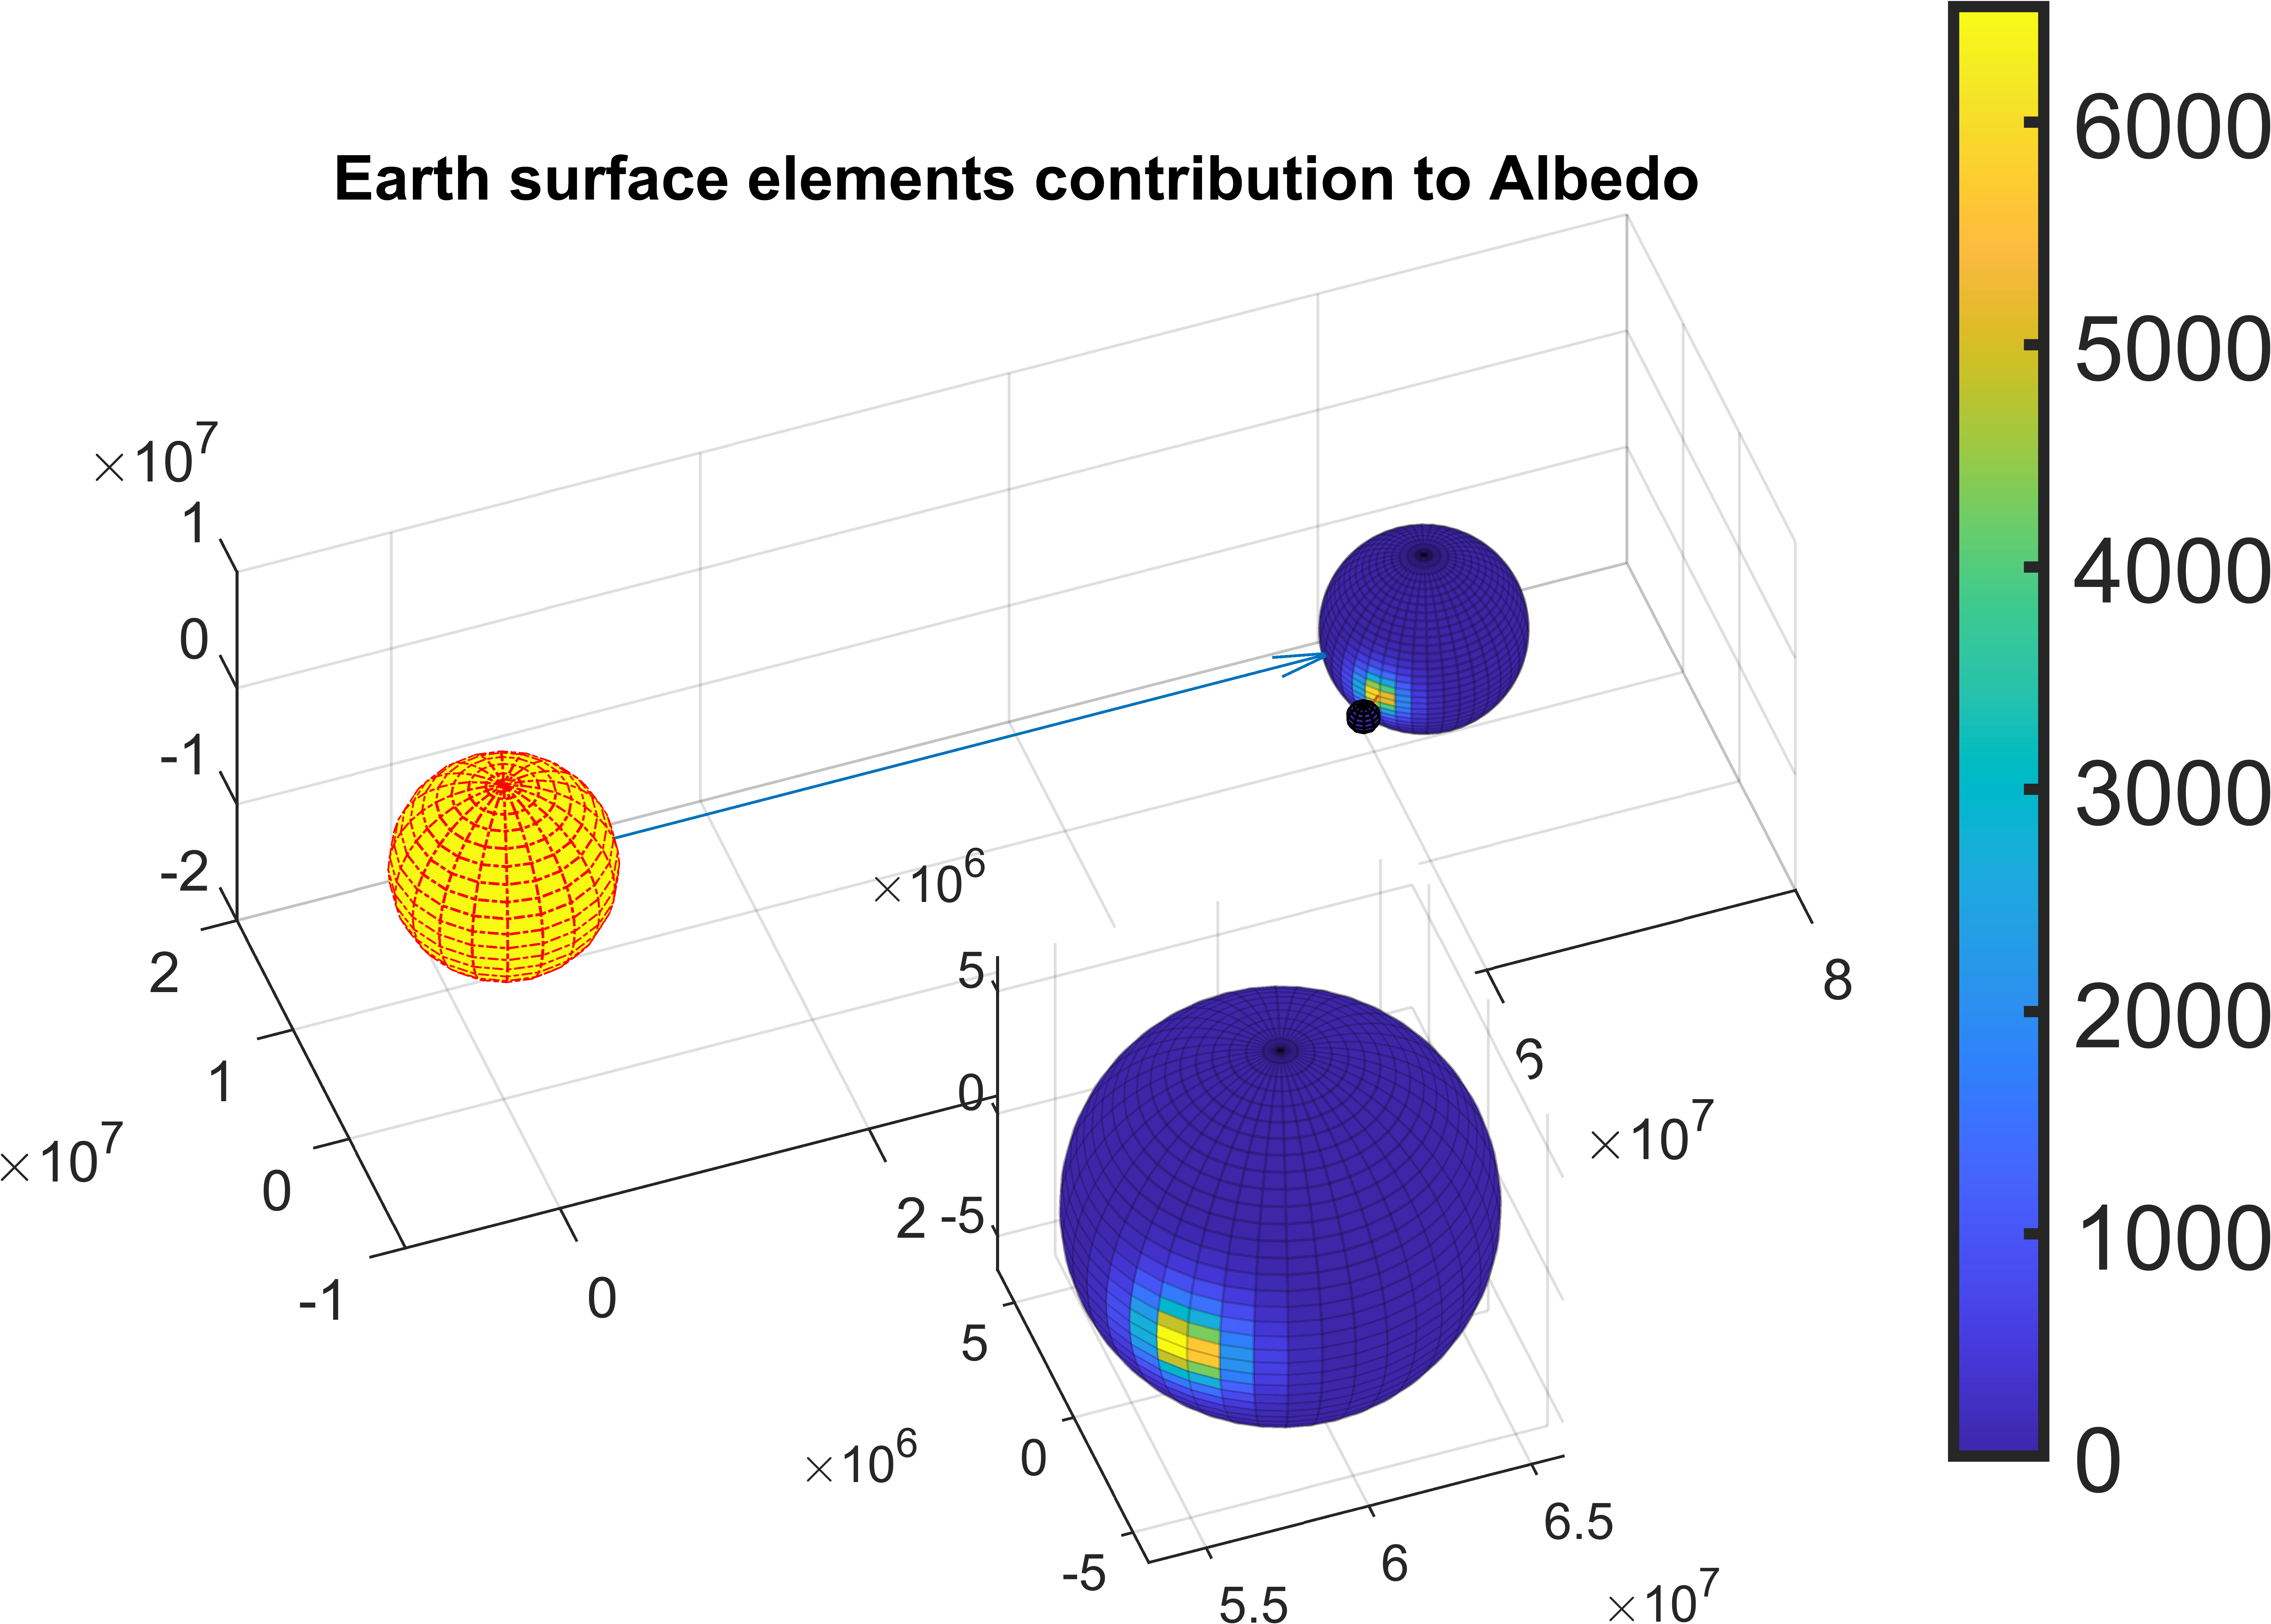
\includegraphics[width=\textwidth]{Matlab/images/albedo_elements.png}
        \caption{}
        \label{fig:albedo}
    \end{subfigure}
    \caption{(a) Earth surface elements contributions to albedo, (b) Earth surface elements contributions to albedo}
\end{figure}


The satellite collects albedo radiation, which is a portion of the incident solar radiation that the earth's surface reflects into space. Figure \ref{fig:albedo} elucidates the contribution of each element on the earth's surface to the satellite-absorbed radiation. It's evident from the figure that the angle between the two surfaces directly influences the amount of contribution. Furthermore, the half-side of the earth that is far from the sun does not contribute to the albedo radiation, which provides a good validation case for our simulation framework.

 \newpage

\paragraph{Temperature variation w.r.t time,}
Figure \ref{fig:temptime} shows the temperature variation over 24 hours period time with a scope of the behavior over around 2 hours period time (satellite periodic time). The satellite temperature varies according to the time periodically and oscillates between a minimum value of \textcolor{red}{X} and a maximum value of Y.  

\paragraph{$Q_{s}$,$Q_{a}$ and $Q_{p}$ variation w.r.t time,}
text

\begin{figure}[H]
    \centering
    \begin{subfigure}[b]{1\textwidth}
        \includegraphics[width=\textwidth]{Matlab/images/temp_time.png}
        \caption{}
        \label{fig:temptime}
    \end{subfigure}
    \begin{subfigure}[b]{1\textwidth}
        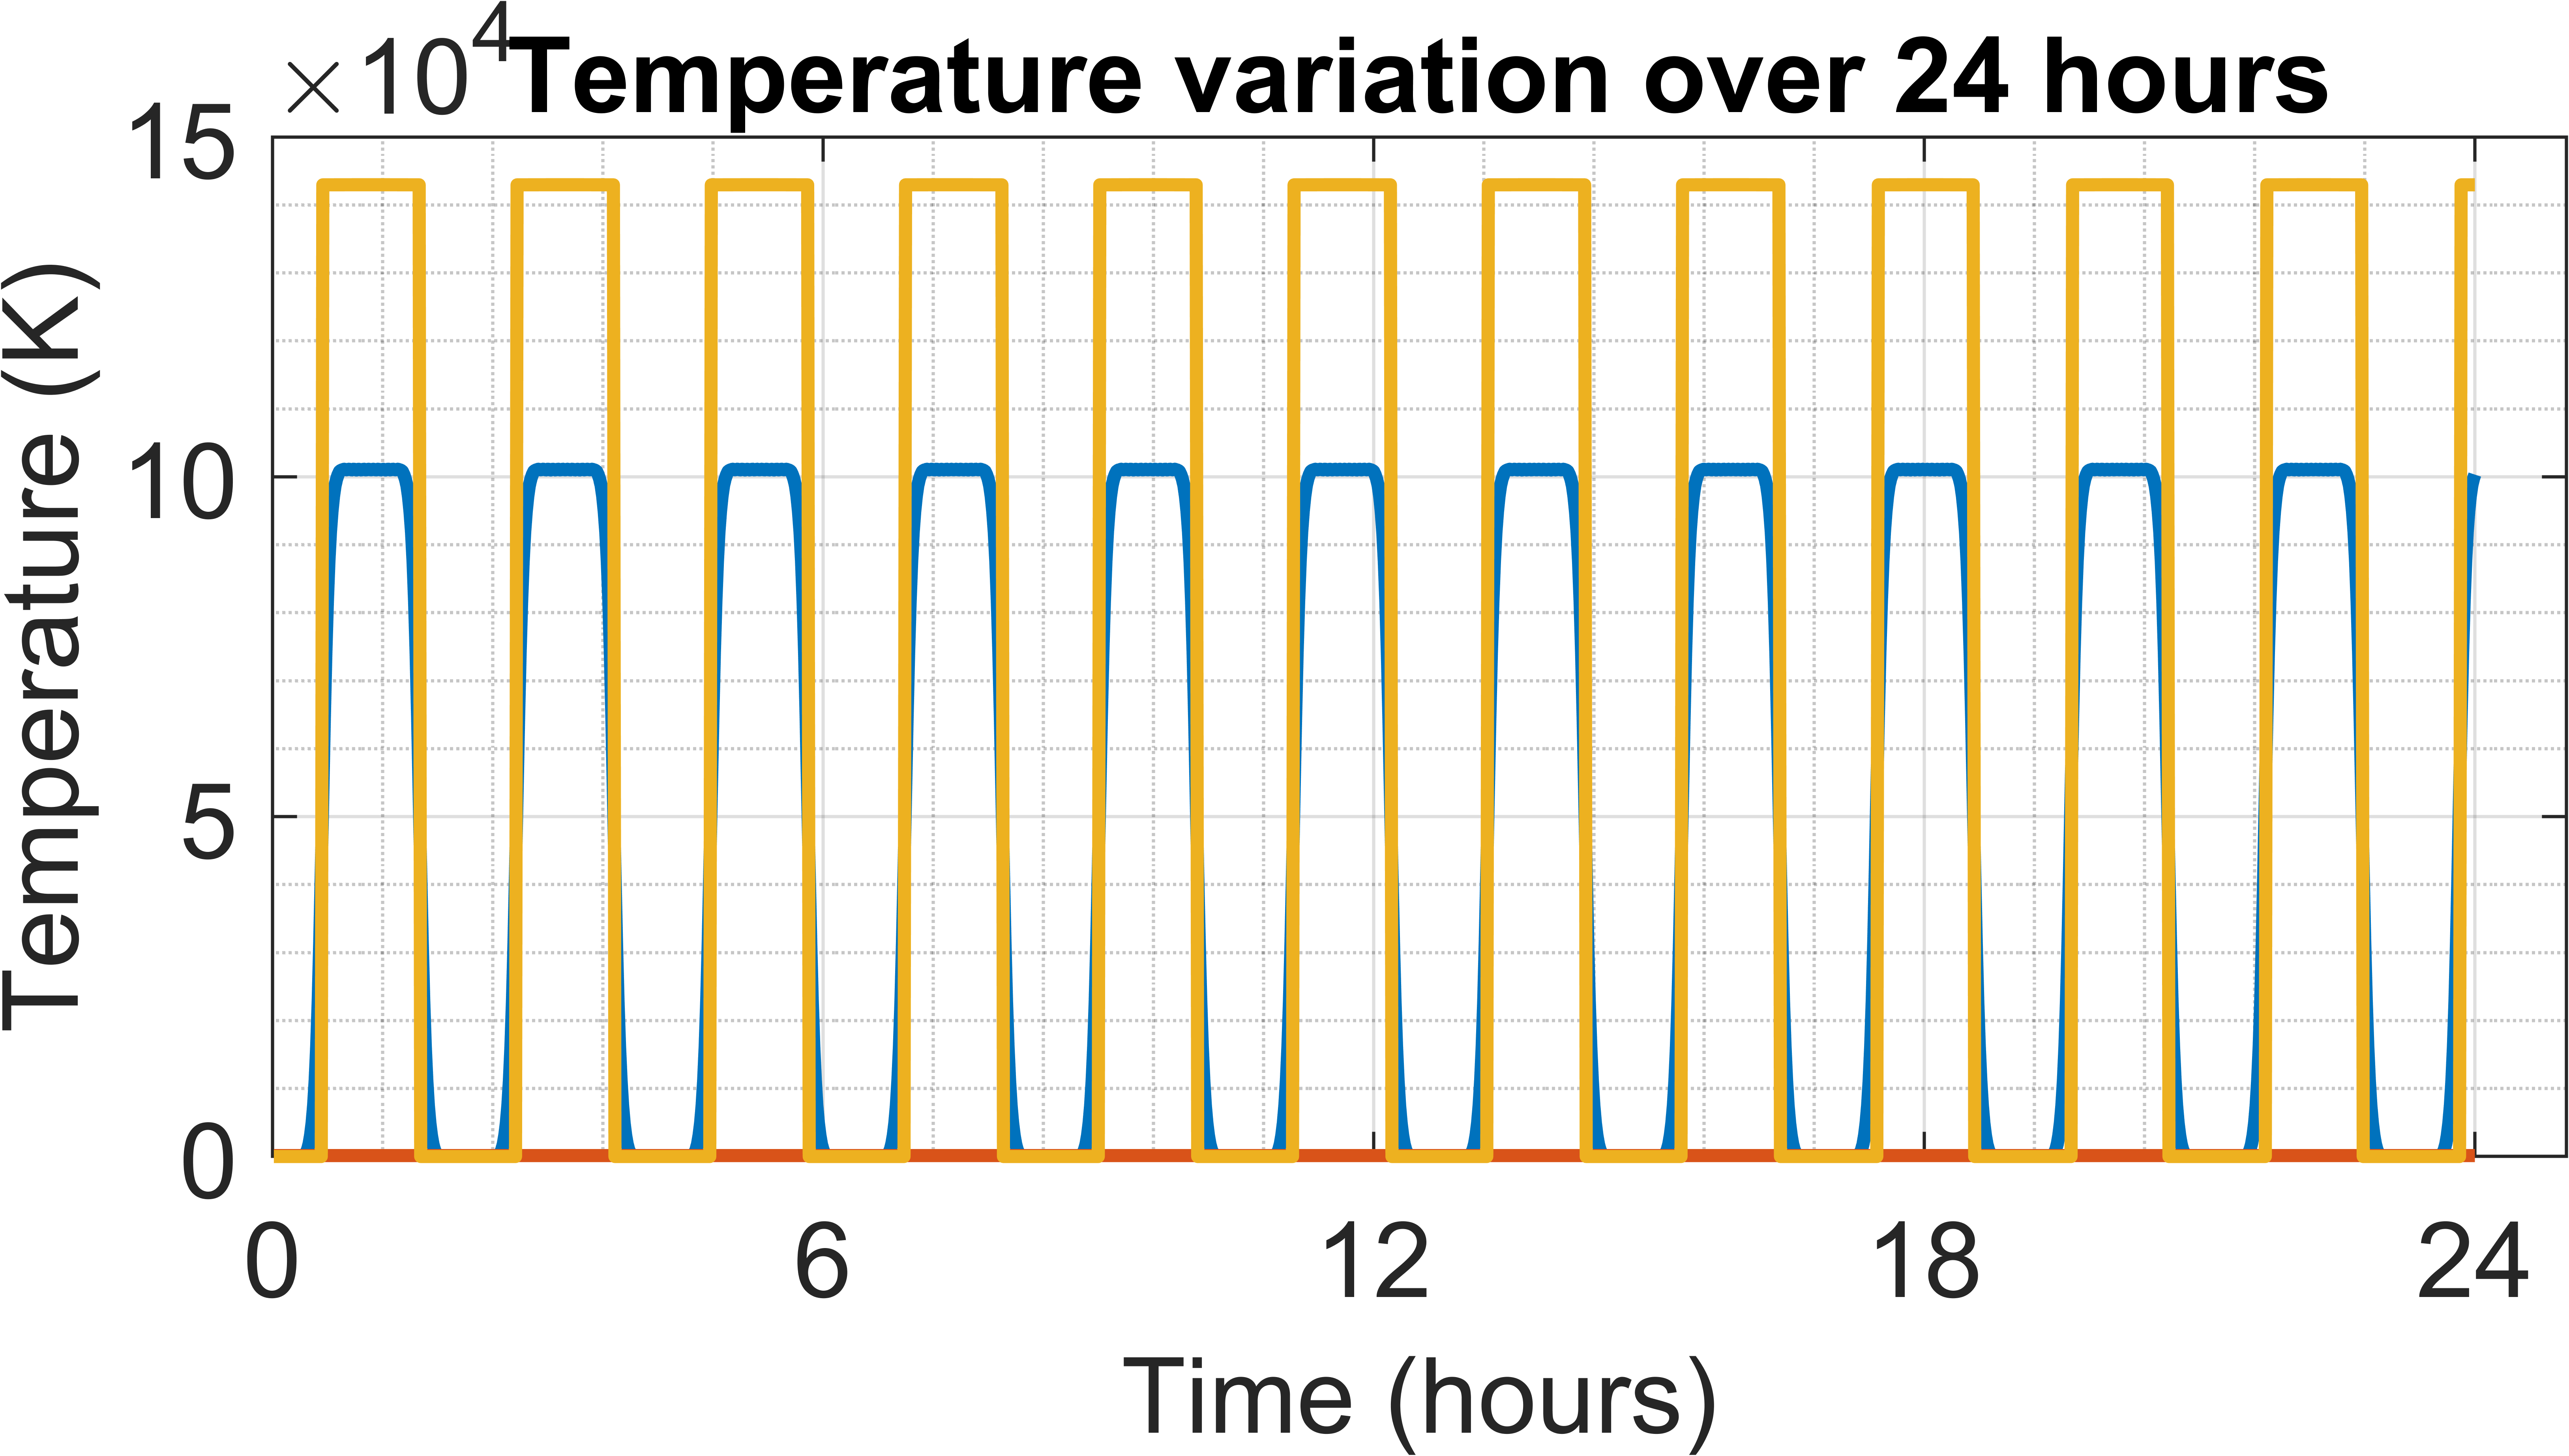
\includegraphics[width=\textwidth]{Matlab/images/QQQ_time.png}
        \caption{}
        \label{fig:temptime}
    \end{subfigure}
    \begin{subfigure}[b]{1\textwidth}
        \includegraphics[width=\textwidth]{Matlab/images/Q_time.png}
        \caption{}
        \label{fig:temptime}
    \end{subfigure}
    \caption{(a) Temperature variation, (b) radiation power variation, and (c) Total incident traditional power to the satellite over time}
\end{figure}







 
FOR EACH MATERIAL (EXCEPT ANIMATIONS)
\begin{enumerate}
    \item Temp variance w.r.t earth-sun period
    \item $Q_{s}$,$Q_{a}$ and $Q_{p}$ variance w.r.t earth-sun period
    \item Temp variance w.r.t Sat-earth period
    \item $Q_{s}$,$Q_{a}$ and $Q_{p}$ variance w.r.t sat-earth period
    \item animation of sat-earth
    \item animation of earth-sun 


\end{enumerate}


\newpage
\section{Discussion} %MSF&IZ
\indent The aforementioned results provide confirmation for the hypothesis that the power assimilated by the satellite diminishes throughout eclipse phases. This phenomenon occurs because albedo and solar radiation are absent during eclipse phases. According to the simulations (refer to figure \ref{fig:temptime}), the satellite completes one revolution around the Earth every 128 minutes, with an eclipse occurring for half of each period. The previously mentioned variation induces a recurring pattern of fluctuations in the overall incident radiation reaching the satellite. This ultimately leads to the recurrence of the effect cycle on the satellite's temperature. As a result of this variation, the satellite constantly oscillates within the temperature range of 205 to 290K. While the temperature range mentioned may not be optimal, it is worth noting that the typical temperature variation for a satellite in Low Earth Orbit (LEO) is between -150 and 60 degrees Celsius \cite{iles2004photovoltaic}. Consequently, this report's results and methodology are validated.

\indent The simulation was executed using different value of $\frac{\alpha}{\epsilon}$, to analyse the effect of different materials on the temperature. It was found that 



\newpage
\section{Conclusion} MSF
\indent






%%%%%%%%%%
%%%%%%%%%%%
%%%%%%%%%%%%
\nomenclature[A, 01]{$\mu$}{\href{https://en.wikipedia.org/wiki/Standard_gravitational_parameter}{Gravitational Parameter} \nomunit{\SI{3.986e14}{\meter\cubed\per\second\squared}}}
\nomenclature[A, 02]{\(Ps\)}{\href{https://en.wikipedia.org/wiki/Standard_gravitational_parameter}{Solar Power}\nomunit{\SI[group-digits=false]{3.856e-26}{\watt}}}
\nomenclature[A, 03]{\(G\)}{\href{https://physics.nist.gov/cgi-bin/cuu/Value?bg}{Gravitational constant} \nomunit{\SI[group-digits=false]{6.67430e-11}{\meter\cubed\per\kilogram\per\second\squared}}}



\nomenclature[B, 03]{\(\mathbb{R}\)}{Real numbers}
\nomenclature[B, 02]{\(\mathbb{C}\)}{Complex numbers}
\nomenclature[B, 01]{\(\mathbb{H}\)}{Quaternions}
\nomenclature[C]{\(V\)}{Constant volume}
\nomenclature[C]{\(\rho\)}{Friction index}






\textcolor{red}{please, add the used constants and abbreviations}


\printnomenclature
\printacronyms
\bibliography{References}

\end{document}

